\documentclass[10pt]{beamer}
\usetheme[
%%% option passed to the outer theme
%    progressstyle=fixedCircCnt,   % fixedCircCnt, movingCircCnt (moving is deault)
  ]{Feather}
  
% If you want to change the colors of the various elements in the theme, edit and uncomment the following lines

% Change the bar colors:
%\setbeamercolor{Feather}{fg=red!20,bg=red}

% Change the color of the structural elements:
%\setbeamercolor{structure}{fg=red}

% Change the frame title text color:
%\setbeamercolor{frametitle}{fg=blue}

% Change the normal text color background:
%\setbeamercolor{normal text}{fg=black,bg=gray!10}

%-------------------------------------------------------
% INCLUDE PACKAGES
%-------------------------------------------------------

\usepackage[utf8]{inputenc}
\usepackage[english]{babel}
\usepackage[T1]{fontenc}
\usepackage{helvet}
\usepackage[justification=centering]{caption}
\usepackage{subcaption}
%\usepackage{multicol}

%-------------------------------------------------------
% DEFFINING AND REDEFINING COMMANDS
%-------------------------------------------------------

% colored hyperlinks
\newcommand{\chref}[2]{
  \href{#1}{{\usebeamercolor[bg]{Feather}#2}}
}

%-------------------------------------------------------
% INFORMATION IN THE TITLE PAGE
%-------------------------------------------------------

\title[ICPRS-18 Conference] % [] is optional - is placed on the bottom of the sidebar on every slide
{ % is placed on the title page
      \textbf{Towards landmarks prediction with Deep Network}
}

%subtitle[The Feather Beamer Theme]
%{
%      \textbf{v. 1.0.0}
%}

\author[V.L. Le, M. Beurton-Aimar, A. Zemmari, N. Parisey]
{      Van-Linh LE$^{1,3}$, Marie BEURTON-AIMAR$^{1}$,\\ Akka ZEMMARI$^{1}$, Nicolas PARISEY$^{2}$ \\[0.4cm]
      {\ttfamily\footnotesize{linhlv@dlu.edu.vn/van-linh.le@labri.fr, beurton@labri.fr\\
		akka.zemmari@labri.fr, nicolas.parisey@inra.fr \\    }
      }
}

\institute[]
{
      $^1$LaBRI-CNRS 5800, Bordeaux University, France\\
      $^2$IGEPP, INRA 1349 Rennes, France\\
      $^3$ITDLU, Dalat University, Vietnam
  
  %there must be an empty line above this line - otherwise some unwanted space is added between the university and the country (I do not know why;( )
}
\date[ICPRS-2018]{\textbf{ICPRS Conference}\\Valparaíso, 22-24 May, 2018}
%\date{\today}

%-------------------------------------------------------
% THE BODY OF THE PRESENTATION
%-------------------------------------------------------

\begin{document}

%-------------------------------------------------------
% THE TITLEPAGE
%-------------------------------------------------------

{\1% % this is the name of the PDF file for the background
\begin{frame}[plain,noframenumbering] % the plain option removes the header from the title page, noframenumbering removes the numbering of this frame only
  \titlepage % call the title page information from above
\end{frame}}

%-------------------------------------------------------

\begin{frame}[t]{Context}
%-------------------------------------------------------
\begin{block}{Morphometry analysis}
  \begin{itemize}    
    \item Used to study the complex interaction between the evolution of insect and environmental factors.
    \item Characterize the common information of biological shape, such as, shape, sizes, or \textbf{landmarks},\ldots.
  \end{itemize}
  \end{block}

  \begin{block}{Landmark}
  \begin{itemize}
     \item A kind of \textbf{point of interest} 
     \item A specific point defined by biologist. For example, intersection of veins on fly wing, the corner of beetle's pronotum,\ldots
  \end{itemize}
  	\begin{figure}[htbp]
       \centering
       \includegraphics[scale=.17]{images/wing}~~~~~~
       \includegraphics[scale=.3]{images/pronotum_lm}~~
	\end{figure}
  \end{block}
\end{frame}

%-------------------------------------------------------

%-------------------------------------------------------

\begin{frame}[c]{Dataset}
%-------------------------------------------------------
	\begin{columns}
		\begin{column}{0.5\textwidth}
			\begin{itemize}
    			\item Images have been taken from $293$ \textbf{beetles}, seperate into 5 parts (images),
    			\item Format: $2$D in RGB color,
    			\item Focus on \textbf{\color{red}pronotum} images.
  			\end{itemize}
		\end{column}
		\begin{column}{0.5\textwidth}  %%<--- here
    		\begin{center}
     			\begin{figure}[htbp]
        			\centering
        			\includegraphics[scale=1]{images/pronotum}
        			%\caption{\footnotesize{Pronotum}}
    				\label{figrsexample1}
				\end{figure}
     		\end{center}
		\end{column}
	\end{columns}~\\
	\begin{figure}[htbp]
   				\begin{subfigure}[t]{0.22\textwidth}
        			\centering
        			\includegraphics[scale=.13]{images/mgmo}
        			\caption{\footnotesize{Left mandible}}
        			\label{figsub11}
    			\end{subfigure}%
    			~ 
    			\begin{subfigure}[t]{0.22\textwidth}
        			\centering
        			\includegraphics[scale=.13]{images/mdmo}
        			\caption{\footnotesize{Right mandible}}
        			\label{figsub22}
    			\end{subfigure}
    			~ 
    			\begin{subfigure}[t]{0.22\textwidth}
        			\centering
        			\includegraphics[scale=.16]{images/elytre2}
        			\caption{\footnotesize{Body}}
        			\label{figsub22}
    			\end{subfigure}
    			~ 
    			\begin{subfigure}[t]{0.22\textwidth}
        			\centering
        			\includegraphics[scale=.16]{images/tete2}
        			\caption{\footnotesize{Head}}
        			\label{figsub22}
    			\end{subfigure}
			\end{figure}
\end{frame}

%-------------------------------------------------------

\begin{frame}{Problems}{}
%-------------------------------------------------------
  
	\small{With un-segmentable images: }
  \begin{figure}[htbp]
        \centering
        \includegraphics[scale=.055]{images/prono_003}
        \pause
         ~~~~~\includegraphics[scale=.055]{images/prono_003_lm}
        %\caption{\footnotesize{Pronotum}}
	\end{figure}
	\textbf{\color{red}How to predict the landmarks coordinates?}
\end{frame}

%-------------------------------------------------------
\begin{frame}{Content}{}
\tableofcontents
\end{frame}
%-------------------------------------------------------
\section{Deep learning and Convolutional Neural Networks}
\subsection{Deep learning}
%-------------------------------------------------------
\begin{frame}{Deep learning}{}
	\only<1-2>{
	\begin{block}{Definition\footnotemark[1]}
		\begin{itemize}
			\item A class of machine learning,
			\item Use a cascade of multiple layers for feature extraction and transformation,
			\item Learn multiple levels of representation in supervised or unsupervised.
		\end{itemize}
	\end{block}{\footnotetext[1]{\tiny{Y. LeCun, Y. Bengio, and G. Hinton, “Deep learning,” Nature, vol. 521, no. 7553, pp. 436–444, 2015}}}
	}
	\only<2>{
	\begin{block}{Applications\footnotemark[1]}
		\begin{itemize}
			\item Computer vision (image recognition and classification)
			\item Speech recognition
			\item Question answering, language translation
		\end{itemize}
	\end{block}
	}
\end{frame}
%-------------------------------------------------------
\subsection{Convolutional neural networks (CNNs)}
%-------------------------------------------------------
\begin{frame}{CNNs}
	\begin{itemize}
		\item Consists an input, an output and multiple hidden layers\footnotemark[1]
		\item Arranges the data in $3$ dimensions: \textit{width, height and depth}
		\item Classical layers: convolutional layers (\textbf{CONV}), pooling layers (\textbf{POOLING}), dropout layers (\textbf{DROPOUT}), full-connected layers (\textbf{FC}), \ldots
	\end{itemize}
	\begin{figure}[htbp]
  		\centering
   	 	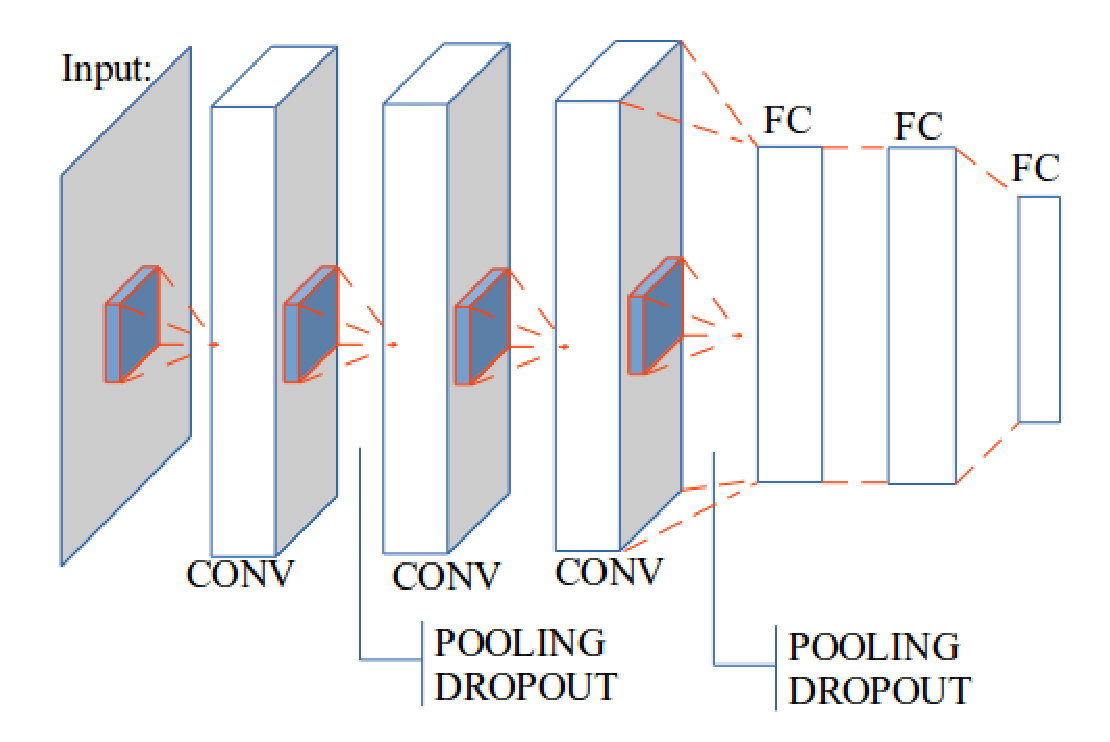
\includegraphics[scale=.35]{images/convarc.eps}
   	 	%\caption{\footnotesize{An example of CNN}}
	\end{figure}
	\footnotetext{
		\tiny{
			Y. LeCun et al, ``Convolutional networks
and applications in vision", 2010.
		}
	}
\end{frame}
%-------------------------------------------------------
\section{Proposed method}
\subsection{Network architectures}
%-------------------------------------------------------
%-------------------------------------------------------
\begin{frame}{Network architecture}{}
  \begin{columns}
		\begin{column}{0.4\textwidth}	
			\only<1>{
			Elementary block: 
			\small{
			\begin{itemize}
				\item A CONV layer,
    			\item A maxixum POOLING layer,
    			\item A DROPOUT layer
  			\end{itemize}}  			
  			}			 			
		\end{column}
		\begin{column}{0.6\textwidth}  %%<--- here
			\only<1>{
			\begin{center}
     			\begin{figure}[htbp]
        			\centering
        			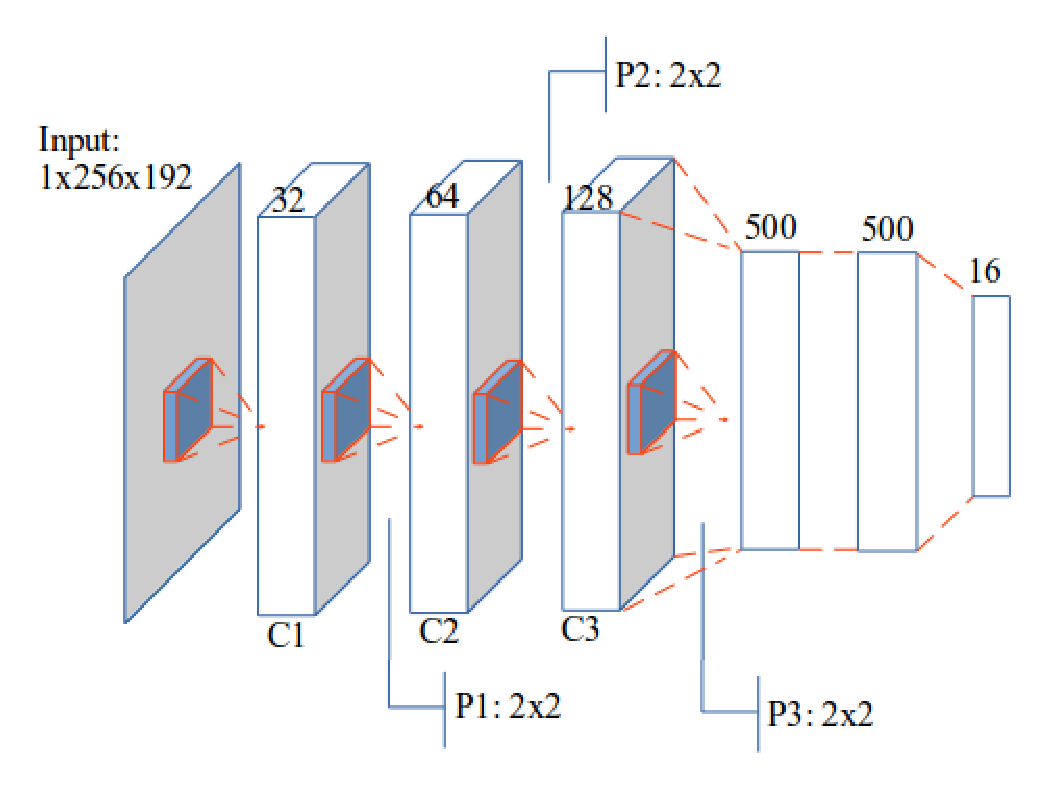
\includegraphics[scale=.4]{images/architecture1}
        			%\caption{\footnotesize{Pronotum}}
    				\label{figrsexample1}
				\end{figure}
     		\end{center}	
     		}					     		
		\end{column}
	\end{columns}~\\
	\only<2>{			
		The proposed model: 
		\small{
			\begin{itemize}
				\item \textbf{Three} elementary blocks,
    			\item \textbf{Three} full-connected (FC) layers
    			\item A dropout layer was inserted between the first of two FCs
  			\end{itemize}}
  		
    		\begin{center}
     			\begin{figure}[htbp]
        			\centering
        			\includegraphics[scale=.2]{images/arch_model}
				\end{figure}
     		\end{center}
     		
		}
\end{frame}
%-------------------------------------------------------
\subsection{Data augmentation}
%-------------------------------------------------------
\begin{frame}{Data augmentation}{}
	\only<1,4>{Dataset: $293$ pronotum images in RGB format.\\}
	\only<2-4>{Augmentation methods:
	\begin{itemize}
		\only<2,4>{\item Increase the value of each channel,}
		\only<3,4>{\item Split the channels.}
	\end{itemize}
	}
	\only<4>{Total: $293 \times 7 = 2,051$ images}
\only<2>{
  \begin{center}
     \begin{figure}[htbp]
        \centering
        \includegraphics[scale=.45]{images/inc_channels}
       	%\caption{\footnotesize{Pronotum}}
    	\label{figrsexample1}
	\end{figure}
  \end{center}
  }
 \only<3>{
  \begin{center}
     \begin{figure}[htbp]
        \centering
        \includegraphics[scale=.45]{images/sp_channels}
       	%\caption{\footnotesize{Pronotum}}
    	\label{figrsexample1}
	\end{figure}
  \end{center}
  }
  \only<4>{
  \begin{center}
     \begin{figure}[htbp]
        \centering
        \includegraphics[scale=.25]{images/data_aug}
       	%\caption{\footnotesize{Pronotum}}
    	\label{figrsexample1}
	\end{figure}
  \end{center}
  }

\end{frame}
%-------------------------------------------------------
\subsection{Training from scratch}
%-------------------------------------------------------
\begin{frame}{Training}{}
	\begin{itemize}
		\item Model: the third model in $5,000$ epochs\footnotemark
		\item Training dataset: $1,820$ images ($260 \times 7$)
		\item Images shows training and validation losses of the models.\\ \small{{\color{blue}Blue} curves are training losses, {\color{green}green} curves are validation losses.}
		\item Training time: 3 hours using NVIDIA TITAN X card.
	\end{itemize}
	\begin{center}
     \begin{figure}[htbp]
        \centering
        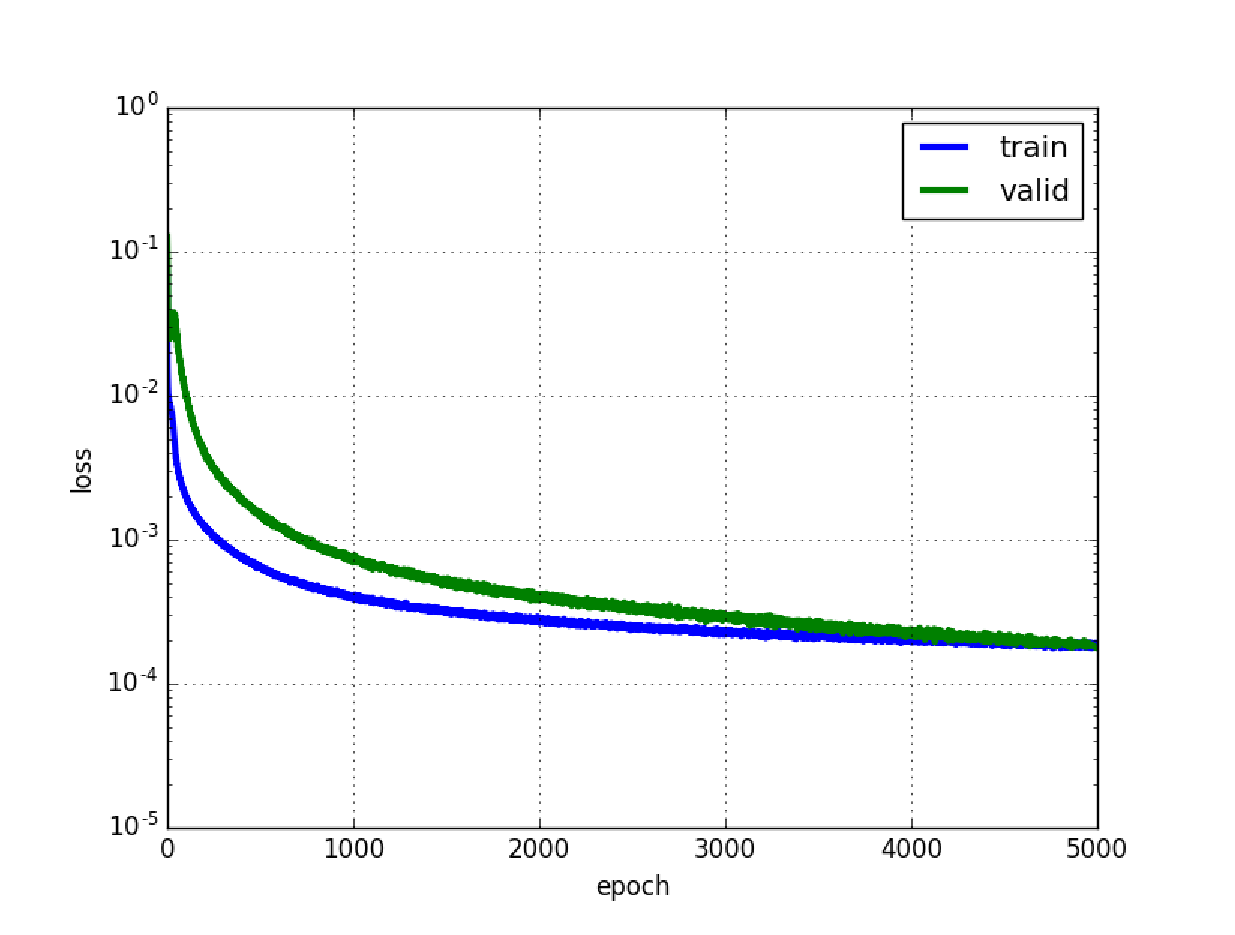
\includegraphics[scale=.31]{images/loss_model_3}
       	%\caption{\footnotesize{Pronotum}}
    	\label{figrsexample1}
	\end{figure}
  \end{center}
	
	\footnotetext{\tiny{An epoch is a single pass through the full training set.}}
\end{frame}

%-------------------------------------------------------
\section{Result}
%-------------------------------------------------------
%-------------------------------------------------------

\begin{frame}{Result}{Landmarks on images}
%-------------------------------------------------------
Images show the result on testing images.
\begin{figure}[htbp]
   				\begin{subfigure}[t]{0.5\textwidth}
        			\centering
        			\includegraphics[scale=.135]{images/plandmark}
        			\caption{ }
        			\label{figsub11}
    			\end{subfigure}%
    			~ 
    			\begin{subfigure}[t]{0.5\textwidth}
        			\centering
        			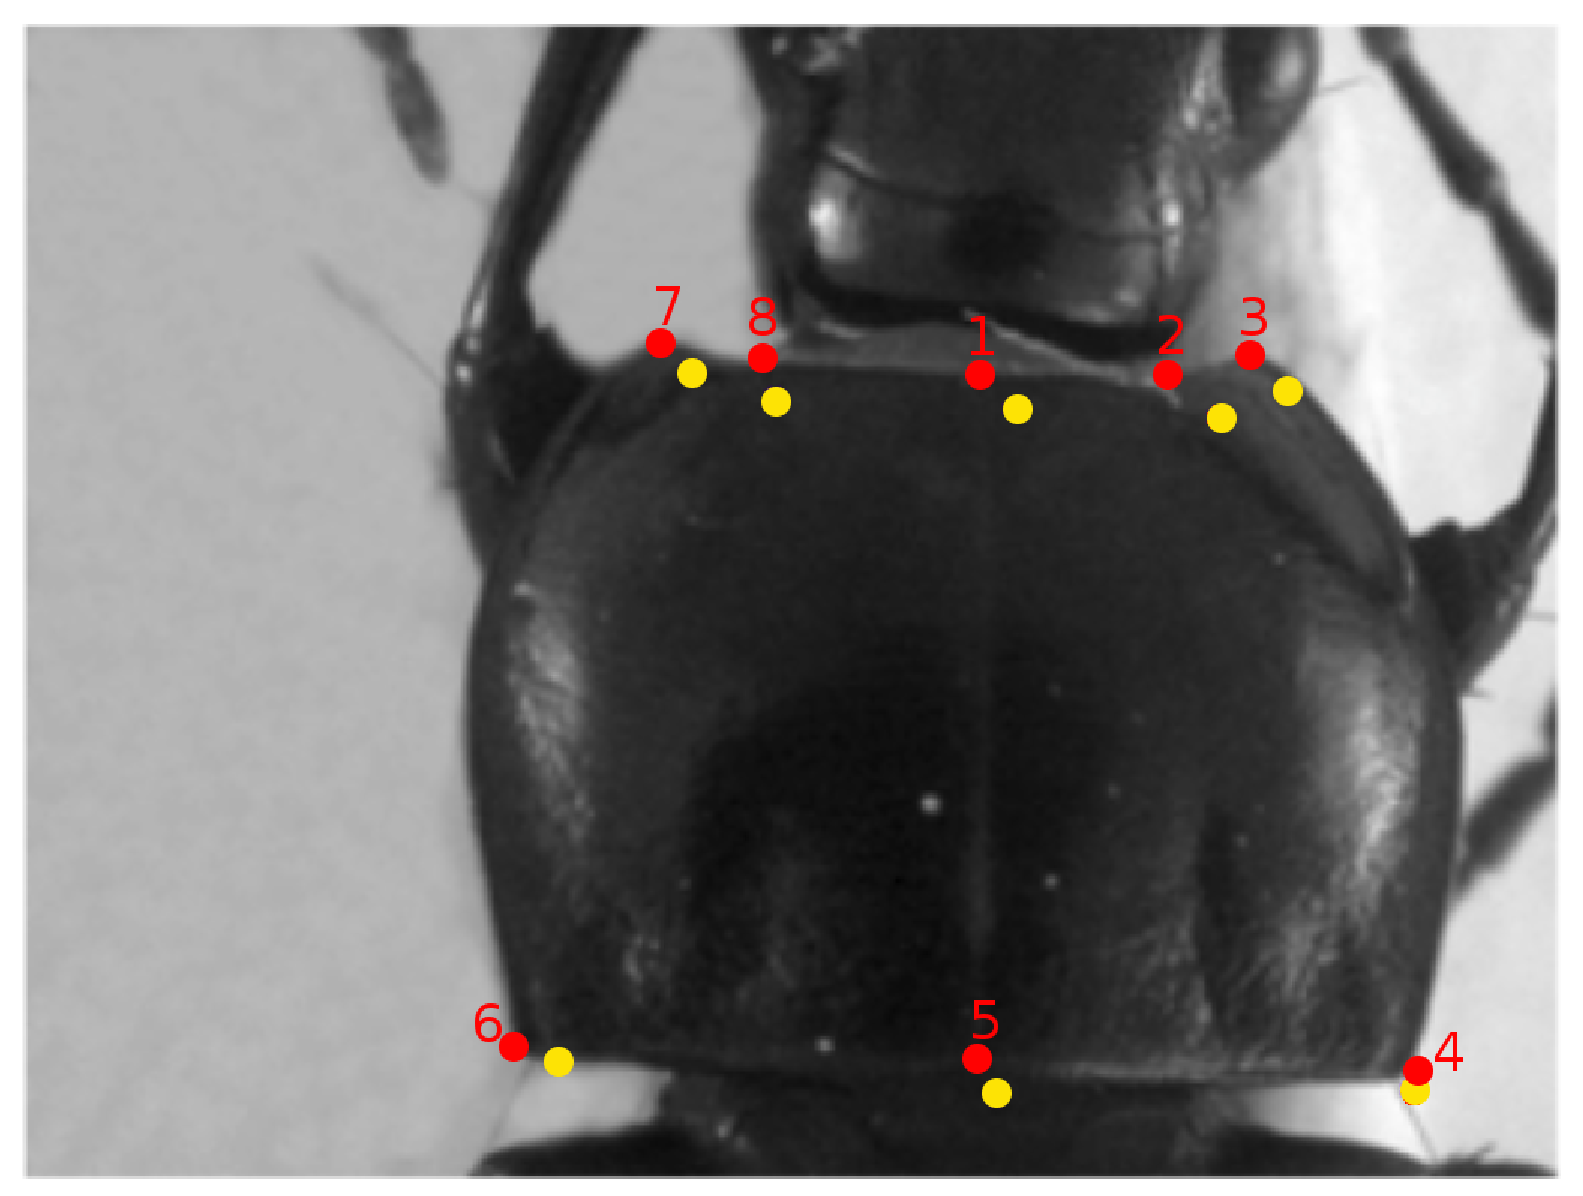
\includegraphics[scale=.2]{images/plandmark2}
        			\caption{ }
        			\label{figsub22}
    			\end{subfigure}    		
    			%\caption{\scriptsize{Training and validation losses of models. Blue curves are training losses, green curves are validation losses.}}	
			\end{figure}
\end{frame}
%-------------------------------------------------------
\begin{frame}{Result}{Average distance}
	\begin{itemize}
		\item Run the trained model to predict the landmarks on testing images,
		\item Calculate the distance between predicted landmarks and corresponding manual landmarks,
		\item Compute the average distance of all images per landmark.
	\end{itemize}
	\begin{center}
		\begin{table}[htbp]
		\centering
		\begin{tabular}{|c|c|}
		\hline
		\textbf{$\#$Landmark} & \textbf{Distance} (in pixels) \\ \hline
			1 & 4.002  \\ \hline
			2 & 4.4831 \\ \hline
			3 & 4.2959 \\ \hline
			4 & 4.3865 \\ \hline
			5 & 4.2925 \\ \hline
			6 & 5.3631 \\ \hline
			7 & 4.636 \\ \hline
			8 & 4.9363 \\ \hline
		\end{tabular}

		\end{table}
	\end{center}
\end{frame}

%-------------------------------------------------------
\subsection{Fine-tuning}
\begin{frame}{Result}{Statistic on acceptable predicted landmarks}
Chart shows the propotion of acceptable predicted landmarks
\footnotesize{
	\begin{itemize}
		\item Average accuracy: $\sim 75\%$
		\item Highest accuracy: $87.88\%$
		\item Lowest accuracy: $66.67\%$
	\end{itemize}
	}
	\begin{figure}[htbp]
		\centering
		\includegraphics[scale=.6]{images/chart2}	
	\end{figure}
\end{frame}
%-------------------------------------------------------
\begin{frame}{Result}{Distribution of distance on the first landmark}
\small{
	\begin{itemize}
		\item Good prediction: $56.66\%$
		\item Acceptable prediction: $40.27\%$
		\item Bad prediction: $3.07\%$
	\end{itemize}
	}
	\begin{figure}[htbp]
		\centering
		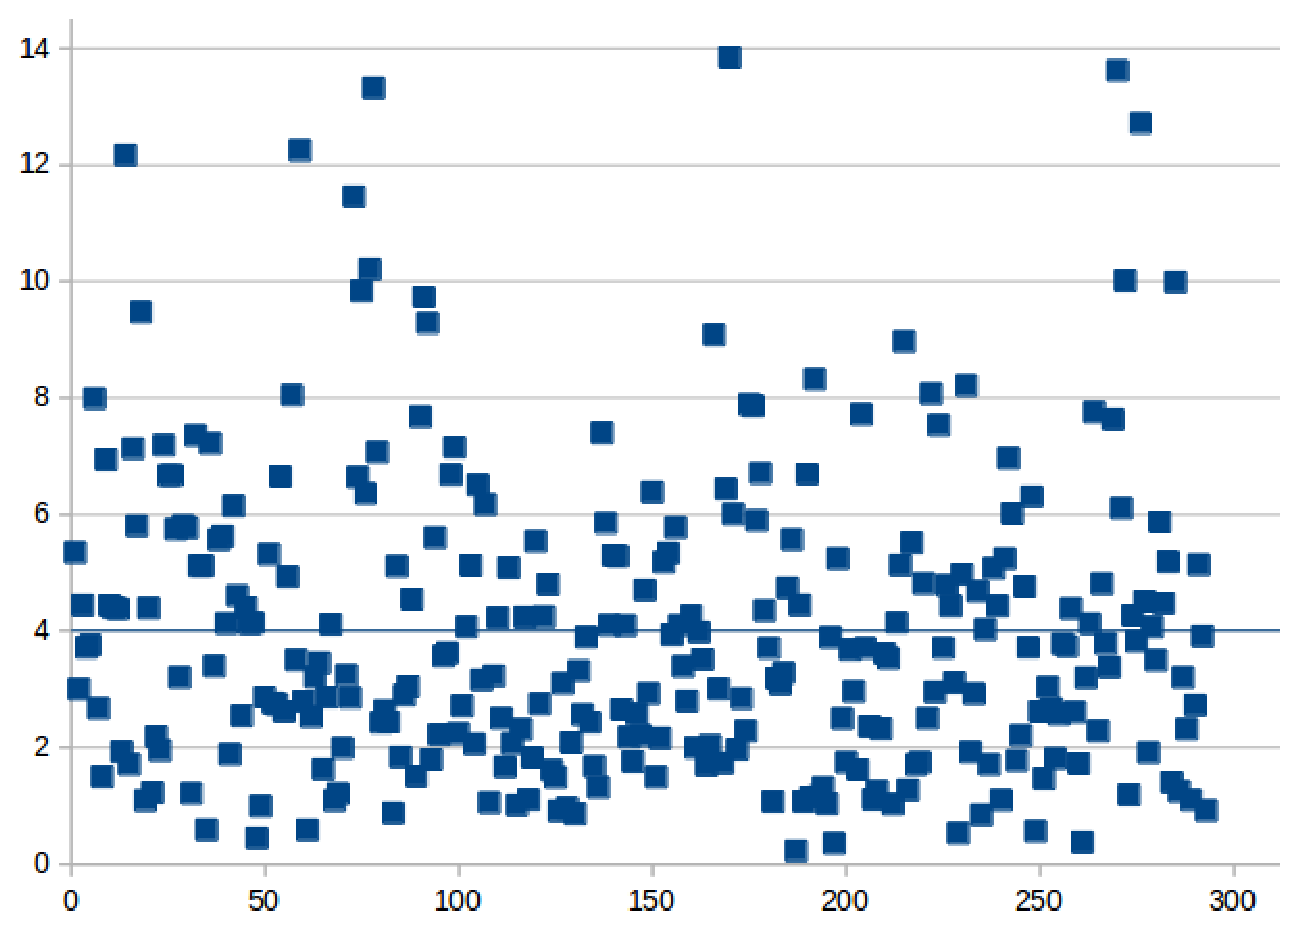
\includegraphics[scale=.3]{images/statistic}	
	\end{figure}
\end{frame}
%-------------------------------------------------------
\begin{frame}{Result}{Comparing with related works}
\small{Quality metrics: coefficient of determination ($r^2$), explained variance (EV), Pearson correlation.
	}
	\begin{table}[htbp]
\centering
\begin{center}
\begin{tabular}{|c|p{1cm}|p{1cm}|p{1.5cm}|}
\hline
Metric & $\mathbf{r^{2}}$ & \textbf{EV} & \textbf{Pearson} \\ \hline
Cintast et al.\footnotemark & $0.884$ & $0.951$ & $0.976$ \\ \hline
Proposed architecture & $\textbf{0.9952}$ & $\textbf{0.9951}$ & $\textbf{0.9974}$ \\ \hline
\end{tabular}
\label{tab3}
\end{center}
\end{table}
\footnotetext{\tiny{Cintas, ``Automatic ear detection and feature extraction using
geometric morphometrics and convolutional neural networks," IET Biometrics, vol. 6, no. 3, pp. 211–223, 2016}}
\end{frame}
%-------------------------------------------------------
\section{Conclusion}
\begin{frame}{Conclusion}
%-------------------------------------------------------
	\begin{block}{Conclusion}
		\small{
			\begin{itemize}
				\item Proposed a CNN to predict the landmarks on pronotum images.
				\item Proposed procedure to augment the dataset.
				\item The location of the predicted landmarks are acceptable with high accuracy ($ \sim75\%$). It allows to replace manual landmarks.
			\end{itemize}
		}
	\end{block}
	\pause
	\begin{block}{Future works}
		\small{Continue improving the landmarks coordinates by continuing on deep learning, \textit{for example}, using transfer learning.}
	\end{block}
\end{frame}
%-------------------------------------------------------

{\1
\begin{frame}[plain,noframenumbering]
  \finalpage{Thank you for attention!}
\end{frame}}

\end{document}





\begin{frame}{Network architecture}
  \begin{columns}
		\begin{column}{0.4\textwidth}
			The first model includes: 
			\small{
			\begin{itemize}
				\item An gray-scale input,
    			\item $3$ CNN layers (C1, C2, C3),
    			\item $3$ POOLING layers (P1,P2,P3),
    			\item $3$ FC layers.
  			\end{itemize}}
  			Problems:
  			\small{
  			\begin{itemize}
  				\item Output is not good enough,
  				\item Overfitting.
  			\end{itemize}
  			}
		\end{column}
		\begin{column}{0.6\textwidth}  %%<--- here
    		\begin{center}
     			\begin{figure}[htbp]
        			\centering
        			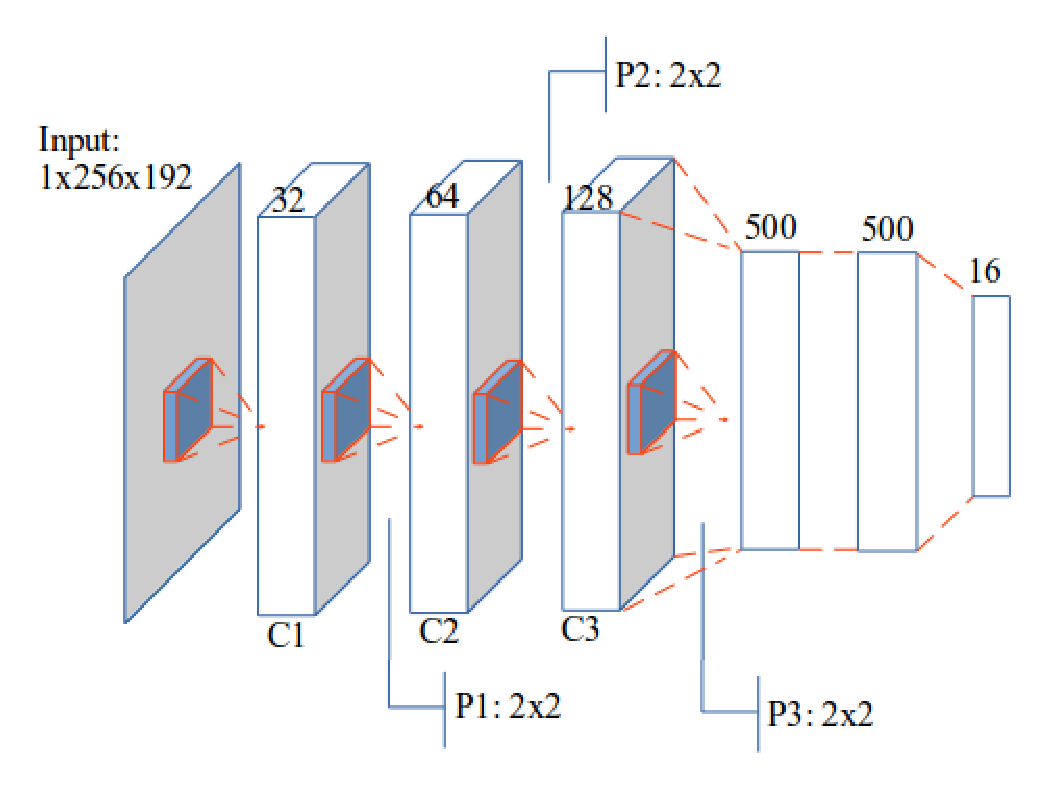
\includegraphics[scale=.4]{images/architecture1}
        			%\caption{\footnotesize{Pronotum}}
    				\label{figrsexample1}
				\end{figure}
     		\end{center}
		\end{column}
	\end{columns}~\\
\end{frame}